\documentclass[a4paper,12pt]{article}
\usepackage{CJKutf8}
\usepackage{amsthm}
\usepackage{amsmath}
\usepackage{amssymb}
\usepackage{geometry}
\usepackage{tikz}
\usetikzlibrary{chains}
\usepackage{subfigure}
\usepackage{enumerate}

% 边距
\geometry{left=2.0cm,right=2.0cm,top=2.0cm,bottom=3.0cm}

\newtheorem{theorem}{Theorem}
\newtheorem{lemma}[theorem]{Lemma}
\newtheorem{proposition}[theorem]{Proposition}
\newtheorem{corollary}[theorem]{Corollary}
\newtheorem{exercise}{Exercise}
\newtheorem*{solution}{Solution}
\newtheorem{definition}{Definition}
\theoremstyle{definition}

\makeatletter \renewenvironment{proof}[1][Proof] {\par\pushQED{\qed}\normalfont\topsep6\p@\@plus6\p@\relax\trivlist\item[\hskip\labelsep\bfseries#1\@addpunct{.}]\ignorespaces}{\popQED\endtrivlist\@endpefalse} \makeatother
\makeatletter
\renewenvironment{solution}[1][Solution] {\par\pushQED{\qed}\normalfont\topsep6\p@\@plus6\p@\relax\trivlist\item[\hskip\labelsep\bfseries#1\@addpunct{.}]\ignorespaces}{\popQED\endtrivlist\@endpefalse} \makeatother

% 大题
\newenvironment{problems}{\begin{list}{}{\renewcommand{\makelabel}[1]{\textbf{##1}\hfil}}}{\end{list}}

% 小题
\newenvironment{steps}{\begin{list}{}{\renewcommand{\makelabel}[1]{\textbf{##1}\hfil}}}{\end{list}}

% 标题
\title{\small \underline{Mathematical Foundations of Computer Science}\\\Large Project 9}
\author{Log Creative\\\small Student ID: }
\date{\today}

\begin{document}
\maketitle

\noindent\textbf{Warmups}

\begin{problems}
    \item[1] What  is  the  smallest  positive  integer  that  has  exactly $k$ divisors,  for $1\leq k\leq 6$?
    \begin{solution}
        \begin{tabular}{c|cccccc}
            $k$ & 1 & 2 & 3 & 4 & 5 & 6 \\
            \hline
            $n$ & 1 & 2 & 4 & 6 & 16 & 12 
        \end{tabular}
    \end{solution} 
    \item[2] Prove that $\gcd (m, n)\cdot\text{lcm} (m, n)=m\cdot n$, and use this identity to express lcm($m, n$) in terms of lcm($n\bmod m, m$), when $n \bmod m\neq 0$. Hint: Use (4.12), (4.14), and (4.15).
    \begin{proof}
        \begin{align*}
            \gcd (m,n) &\cdot \text{lcm}(m,n) \\
            =& p_1^{\min(m_1,n_1)}p_2^{\min(m_2,n_2)}\cdots p_k^{\min(m_k,n_k)}\cdot&& \text{(By (4.14))}\\
            &p_1^{\max(m_1,n_1)}p_2^{\max(m_2,n_2)}\cdots p_k^{\max(m_k,n_k)} && \text{(By (4.15))}\\
            =&p_1^{\min(m_1,n_1)+\max(m_1,n_1)}p_2^{\min(m_2,n_2)+\max(m_2,n_2)}\cdots p_k^{\min(m_k,n_k)+\max(m_k,n_k)}\\
            =&p_1^{m_1+n_1}p_2^{m_2+n_2}\cdots p_k^{m_k+n_k}\\
            =&m\cdot n &&\text{(By (4.12))}
        \end{align*}

        \begin{align*}
            \text{lcm}(m,n)&= \frac{m\cdot n}{\gcd (m,n)}\\
            &= \frac{m\cdot n}{\gcd (n \bmod m,m)}\\
            &= \frac{m\cdot n}{\frac{m(n\bmod m)}{\text{lcm}(n\bmod m,m)}}\\
            &=\frac{m\cdot n}{n\bmod m}\cdot\text{lcm}(n\bmod m,m) &&(n\bmod m\neq 0)
        \end{align*}
    \end{proof} 
    \item[3] Let $\pi(x)$ be the number of primes not exceeding $x$.  Prove or disprove: $\pi(x) -\pi(x-1) =$ [$x$ is prime].
    \begin{proof}
        It only holds for $x$ is an integer. $x$ could be a real number. In fact,
        \begin{equation*}
            \pi(x) -\pi(x-1) = [\lfloor x \rfloor\text{ is prime}]
        \end{equation*}
        You can only count primes up to $\lfloor x \rfloor$. And if $\lfloor x\rfloor $ is a prime, $x-1$ will ignore this prime, thus the gap 1. Otherwise, no prime is ignored.
    \end{proof} 
    \item[4] What would happen if the Stern-Brocot construction started with the five fractions $\left(\frac{0}{1},\frac{1}{0},\frac{0}{-1},\frac{-1}{0},\frac{0}{1}\right)$ instead of with $\left(\frac{0}{1},\frac{1}{0}\right)$?
    \begin{solution}
        All fractions $m/n$ with $m\vert n$ are constructed.

        $\left(\frac{0}{-1},\frac{-1}{0}\right)$ will give the negative part fractions. Initial Stage always give:
        \begin{align*}
            1\times 1 - 0 \times 0 &= 1\\
            0\times 0 - 1 \times (-1) &= 1\\
            (-1)\times (-1) - 0 \times 0 &= 1 \\
            0\times 0 - (-1)\times 1 &= 1
        \end{align*}
        which satisfies the requirement of 
        \begin{equation*}
            m^\prime n - mn^\prime = 1
        \end{equation*}
        and the chain reaction will continue.
    \end{solution} 
    \item[5] Find simple formulas for $L^k$ and $R^k$, when $L$ and $R$ are the 2$\times$2 matrices of (4.33).
    \begin{solution}
        \begin{equation*}
            L^k=\begin{pmatrix}
                1 & k\\
                0 & 1
            \end{pmatrix}\quad
            R^k=\begin{pmatrix}
                1 & 0\\
                k & 1
            \end{pmatrix}
        \end{equation*}
        
        \textbf{Prove by mathematical induction.}
        \paragraph{Basic steps.}
        \begin{equation*}
            L=\begin{pmatrix}
                1 & 1\\
                0 & 1
            \end{pmatrix}\quad
            R=\begin{pmatrix}
                1 & 0\\
                1 & 1
            \end{pmatrix}
        \end{equation*}

        \paragraph{Induction.} Assumming that 
        \begin{equation*}
            L^{k-1}=\begin{pmatrix}
                1 & k-1\\
                0 & 1
            \end{pmatrix}\quad
            R^{k-1}=\begin{pmatrix}
                1 & 0\\
                k-1 & 1
            \end{pmatrix}
        \end{equation*}
        Then, 
        \begin{align*}
            L^k=L^{k-1}L=\begin{pmatrix}
                1 & k-1\\
                0 & 1
            \end{pmatrix}\begin{pmatrix}
                1 & 1\\
                0 & 1
            \end{pmatrix}=\begin{pmatrix}
                1 & k\\
                0 & 1
            \end{pmatrix}\\
            R^k=R^{k-1}R=\begin{pmatrix}
                1 & 0\\
                k-1 & 1
            \end{pmatrix}\begin{pmatrix}
                1 & 0\\
                1 & 1
            \end{pmatrix}=\begin{pmatrix}
                1 & 0\\
                k & 1
            \end{pmatrix}
        \end{align*}

        As a result, it holds for all $n\in\mathbb{N}_+$.

    \end{solution} 
    \item[6] What does `$a \equiv b\pmod 0$' mean?
    \begin{solution}
        Based on (4.36):
        \begin{equation*}
            a \equiv b\pmod 0 \Leftrightarrow a-b\text{ is a multiple of }0
        \end{equation*}
        Thus,
        \begin{equation*}
            a=b
        \end{equation*}
    \end{solution}
    \item[7] Ten people numbered 1 to 10 are lined up in a circle as in the Josephus problem,  and every mth person is executed.  (The value of $m$ may be much larger than 10.)  Prove that the first three people to go cannot be 10, $k$, and $k+1$ (in this order), for any $k$.
    \begin{proof}
        \textbf{Prove by contradiction.} If the first three people to go is 10, $k$, and $k+1$. 
        
        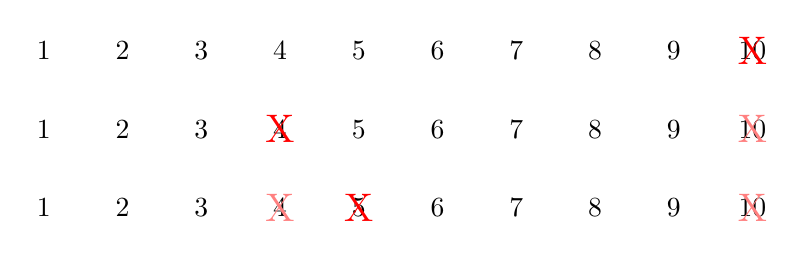
\begin{tikzpicture}
\foreach \x in {1,...,10}
	\foreach \y in {1,2,3}
		\node at (\x,\y) {\x};

\node[red,font=\Large] at (10,3) {X};
\node[red!50,font=\Large] at (10,2) {X};
\node[red!50,font=\Large] at (10,1) {X};
\node[red,font=\Large] at (4,2) {X};
\node[red!50,font=\Large] at (4,1) {X};
\node[red,font=\Large] at (5,1) {X};
\end{tikzpicture}


        The first step implies that 
        \begin{equation*}
            m \bmod 10 = 0
        \end{equation*}

        The second step implies that
        \begin{equation*}
            m \bmod 9 = k
        \end{equation*}

        The third step implies that 
        \begin{equation*}
            m \bmod 8 = 1
        \end{equation*}
        A contradiction comes to $m$ can not be both even and odd from the first step and the third step.
    \end{proof}
\end{problems}

\noindent\textbf{Basics}

\begin{problems}
    \item[14] Prove or disprove:
    \begin{enumerate}[a.]
        \item gcd($km, kn$) =$k$gcd($m, n$)
        \begin{proof}
            When $k$ is a positive integer, the statement is true. Let
            \begin{align*}
                m &= p_1^{\alpha_1}\cdots p_k^{\alpha_k}\\
                n &= p_1^{\beta_1}\cdots p_k^{\beta_k}\\
                \text{gcd}(m,n) &= p_1^{\gamma_1}\cdots p_k^{\gamma_k}
            \end{align*} 
            where $\gamma_i = \min(\alpha_i,\beta_i)$. If
            \begin{equation*}
                k = p_1^{\theta_1}\cdots p_k^{\theta_k}
            \end{equation*}
            Then,
            \begin{align*}
                \gcd(km,kn) &= p_1^{\min(\alpha_1+\theta_1,\beta_1+\theta_1)}\cdots p_k^{\min(\alpha_k+\theta_k,\beta_k+\theta_k)}\\
                &= p_1^{\min(\alpha_1,\beta_1)}\cdots p_k^{\min(\alpha_k,\beta_k)}p_1^{\theta_1}\cdots p_k^{\theta_k}\\
                &= k\gcd(m,n)
            \end{align*}
        \end{proof}
        \item lcm($km, kn$) =$k$lcm($m, n$)
        \begin{proof}
            When $k$ is a positive integer, the statement is true. Let
            \begin{align*}
                m &= p_1^{\alpha_1}\cdots p_k^{\alpha_k}\\
                n &= p_1^{\beta_1}\cdots p_k^{\beta_k}\\
                \text{lcm}(m,n) &= p_1^{\gamma_1}\cdots p_k^{\gamma_k}
            \end{align*} 
            where $\gamma_i = \max(\alpha_i,\beta_i)$. If
            \begin{equation*}
                k = p_1^{\theta_1}\cdots p_k^{\theta_k}
            \end{equation*}
            Then,
            \begin{align*}
                \text{lcm}(km,kn) &= p_1^{\max(\alpha_1+\theta_1,\beta_1+\theta_1)}\cdots p_k^{\max(\alpha_k+\theta_k,\beta_k+\theta_k)}\\
                &= p_1^{\max(\alpha_1,\beta_1)}\cdots p_k^{\max(\alpha_k,\beta_k)}p_1^{\theta_1}\cdots p_k^{\theta_k}\\
                &= k\text{lcm}(m,n)
            \end{align*}
        \end{proof}
    \end{enumerate}

    \item[15] Does every prime occur as a factor of some Euclid number $e_n$?
    \begin{solution}
        No. For example,
        \begin{align*}
            e_1 \bmod 5 &= 2\\
            e_2 \bmod 5 &= 3\\
            e_3 \bmod 5 &= 2\\
            e_4 \bmod 5 &= 3\\
            \cdots
        \end{align*}
        In fact, because $e_n\neq 5$, if $e_n\bmod 5=0$, then $e_n$ is not a prime, which contradicts the property of $e_n$ as a prime.
    \end{solution} 
\end{problems}

\end{document}
